%!TEX root = ../notas_de_clase.tex

\section{Clasificación}
\label{cap:clasificacion}

El problema de clasificación dice relación con la identificación del conjunto, categoría o \emph{clase} a la cual pertenece un elemento en base a sus \emph{características} o \textit{features}. En el contexto del aprendizaje supervisado, el problema de clasificación puede ser visto como un caso particular del problema de regresión, donde el espacio en el que vive la variable $y$ (salida o variable dependiente) es \emph{categórico} y usualmente denotado por $\{0,1\}$, para el caso binario, o bien $\{1,2,\ldots,K\}$ para el caso de clasificación multiclase. 
	
\subsection{\texorpdfstring{$k$} vecinos más cercanos (KNN)}
Dado un conjunto de datos
\begin{equation}
	 	\datos = \{(x_i,c_i)\}_{i=1}^N\subset\R^M\times\{\cC_i\}_{i=1}^K
\end{equation}
donde, al igual que en el problema de regresión, $x$ es la variable independiente y $c$ es la variable dependiente o \emph{clase}, una forma natural de clasificar una nueva entrada $x_\star$ será asignarle la clase correspondiente a los datos observados más similares a $x_\star$. 

Así, el modelo KNN funciona bajo esta lógica:  que entradas similares tienen salidas similares. Bajo este modelo, la formulación del problema de clasificación es la siguiente:\\

Sea $N_k(x_\star)\subset \mathcal{D}$ conjunto de los $k$ vecinos más cercanos a $x_\star$, es decir:

\begin{equation}
	|N_k(x_\star)|=k\quad\text{y}\quad d(x_\star,x)\geq \max_{(x',y')\in N_k(x_\star)} d(x_\star,x'),\quad\forall (x,y)\in \mathcal{D}\backslash N_k(x_\star)
\end{equation}

Donde $d:\R^M\times\R^M\to\R_+$ corresponde a la métrica euclidiana.\\

Entonces, el clasificador KNN retorna la etiqueta más común:

\begin{equation}
	\mathcal{C}(x) = \text{moda}\left(\{y':(x',y')\in N_k(x_\star)\}\right)
\end{equation}

Si bien KNN pareciera un algoritmo heurístico, tiene fuertes propiedades de convergencia. Para enunciar esto, es necesaria la siguiente definición:

\begin{definition}[clasificador óptimo de Bayes]
	dado $p(y|x)$, el clasificador óptimo de Bayes asigna la etiqueta más probable:
	
	\begin{equation}
		\overline{\mathcal{C}}(x)=\argmax_{y\in \{\cC_i\}_{i=1}^K} p(y|x)
	\end{equation}
\end{definition}

En el clasificador anterior, la probabilidad de error corresponde a $e = 1 - p(\overline{\mathcal{C}}|x)$ y es una cota inferior para el error ya que ningún otro clasificador puede obtener un error menor. Dado que no se conoce $p(y|x)$, esta cota corresponde a una cota asintótica.\\

Por otra parte, para el clasificador KNN se tiene el siguiente resultado:

\begin{theorem}[desigualdad de Cover-Hart] sea $R^*$ el error (riesgo) del clasificador óptimo de Bayes y $R$ el error asintótico de KNN, entonces $R$ está acotado, más aún:

\begin{equation}
	R^*\leq R\leq 2R^*(1-R^*)
\end{equation}
	
\end{theorem}

Sin embargo, aunque asintóticamente el clasificador funciona bien, la convergencia a dicha tasa de error es lenta y se ve afectada por la dimensión de la entrada (ver maldición de la dimensionalidad). Es por esto que es necesario formular otros clasificadores bajo otra perspectiva.


\subsection{Clasificación lineal}
\label{sec:clasif_lineal}

\noindent\begin{minipage}{0.52\textwidth}

	  Consideraremos en primera instancia el caso \emph{binario}, es decir, solo dos clases ($K=2$), ilustrado en la Fig.~\ref{fig:puntos_2d}. Proponemos un modelo lineal para relacionar la variable independiente con su clase, es decir, 
	\begin{equation}
		y(x) = a^\top  x + b,
		\label{eq:clasificacion_lineal}
	\end{equation}
	donde la  asignación de la clase es de la siguiente forma: $x$ será asignado a $\cC_1$ si $y(x) \geq 0$ y será asignado $\cC_2$ en caso contrario.\\
	
	Nos referiremos al subconjunto que particiona $\R^M$ en clase $\cC_1$ y clase $\cC_2$ como \emph{superficie/hiperplano/región de decisión}, la cual está definida por $y(x)=0$. Entonces, como $x\in\R^M$, para la consideración del modelo lineal esta superficie de decisión corresponde a un hiperplano de dimensión $M-1$.
\end{minipage}\hfill
%[AGREGAR IMAGEN]
\begin{minipage}{0.46\textwidth}
	\centering
	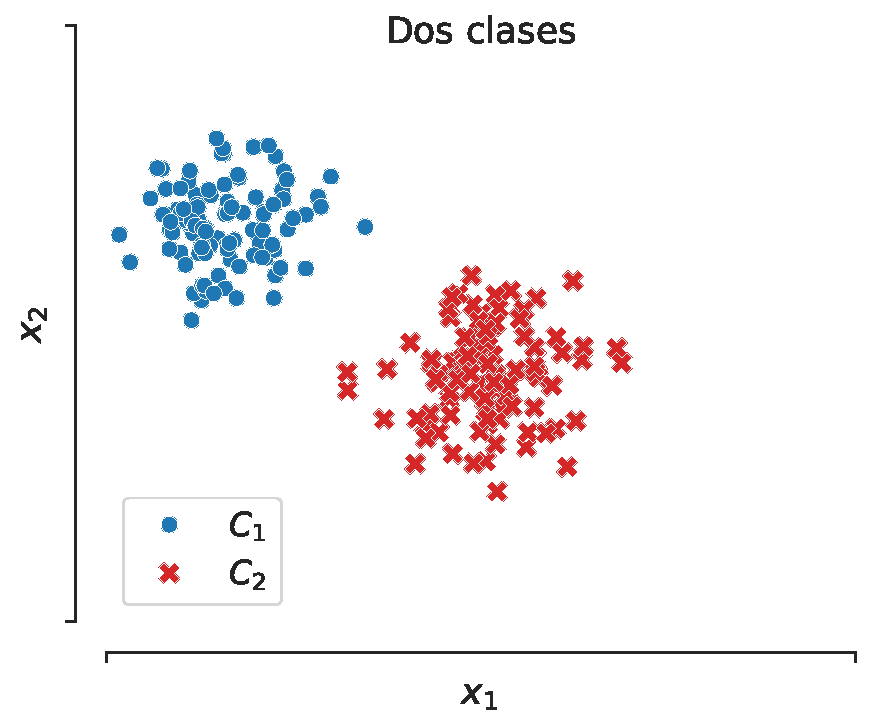
\includegraphics[width=\textwidth]{img/cap3_dosclases}\\
	\captionof{figure}{Ejemplo del problema  de clasificación binaria, donde la clase $\cC_1$ está presentada en azul y la clase $\cC_2$ en rojo.}
	\label{fig:puntos_2d}
\end{minipage}

\vspace{1cm}


Para resolver el problema de clasificación, debemos encontrar los parámetros $a$ y $b$ en la ec.~\eqref{eq:clasificacion_lineal}. Para este fin, veamos que si $x_1,x_2$ son dos puntos en la superficie de decisión, entonces tenemos la siguiente relación para el parámetro $a$:
\begin{align}
	0 &= y(x_1) - y(x_2) \nonumber\\
	  &= a^\top x_1 + b - a^\top x_2 - b \nonumber\\
	  &= a^\top (x_1-x_2).
\end{align}

Es decir, $a$ es ortogonal a cualquier vector que esté contenido dentro de la región de decisión (ya que $x_1-x_2$ corresponde a un vector director del hiperplano). Intuitivamente, podemos decir que el vector $a\in\R^M$ controla la pendiente (o inclinación) del hiperplano de decisión. Además, observemos que para cualquier $x$ en la región de decisión, i.e., $y(x)=0$,  su proyección en el vector $a$ está dada por 
	
	\begin{equation}
	\norm{\text{proy}_a(x)} = \norm{x}cos(\theta) = \norm{x} \frac{a^\top x}{\norm{a}\cdot\norm{x}} = -\frac{b}{\norm{a}}
\end{equation}


\begin{figure}[h]
    \centering
    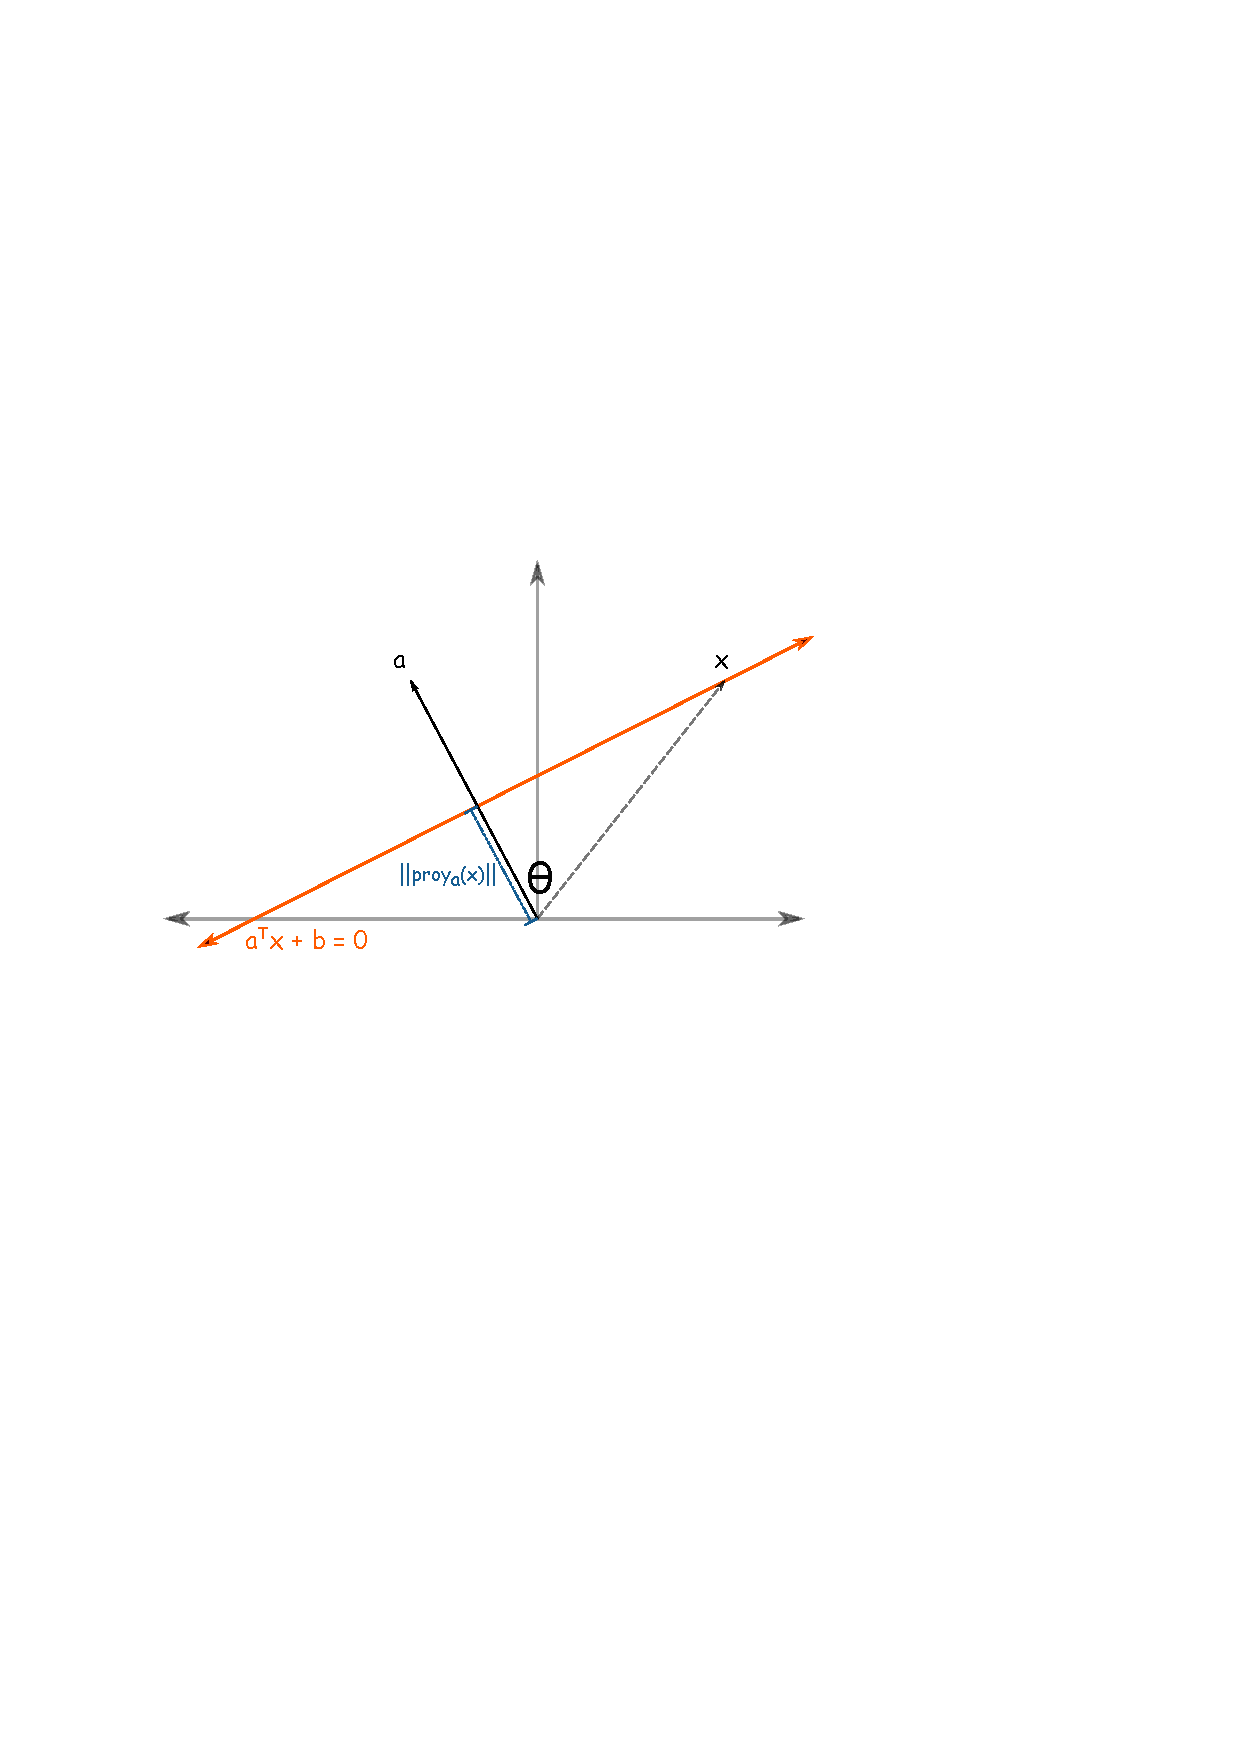
\includegraphics[width=0.5\textwidth]{img/cap3_proy.pdf}
    \caption{Proyección de un punto sobre la región de decisión. }
\end{figure}

Donde se usó el hecho de que $\cos\left(\measuredangle(x,y)\right) = \frac{\langle x,y\rangle}{\norm{x}\norm{y}}$.


Por lo tanto, se concluye que el parámetro $b$ controla el desplazamiento (o ubicación) de la región de decisión,  pues el lado izquierdo de la ecuación representa la distancia entre la región de decisión y el origen: $\norm{\text{proy}_a(x)} = d(\{x:a^\top x+b = 0\},0)$.\\

Es posible  también interpretar $y(x)$ como una distancia con signo entre un $x\in\R^M$ cualquiera  y la superficie de decisión. Para ver esto, consideremos $x\in\R^M$ y descompongámoslo dos componentes: la primera denotada por $x_{\bot}$, la cual es la proyección ortogonal de $x$ en el hiperplano de  decisión, y la segunda que es perpendicular al hiperplano (y consecuentemente paralela al vector $a$) denotada por $r\frac{a}{\left \| a \right \|}$, donde $r$ denota la distancia entre $x$ y el  hiperplano de  decisión. Expresamos entonces  
\begin{equation}
	x = x_{\bot}+r\frac{a}{\left \| a \right \|},
\end{equation}
y observamos que
\begin{equation}
	y(x) 
	= a^\top x+b 
	=a^\top  \left( x_{\bot} + r\frac{a}{\left \| a \right \|} \right) +b 
	= \underbrace{a^\top x_{\bot} +b }_{=0} +   r\frac{a^\top  a}{\left \| a \right \|}
	= r||a||.
\end{equation}
Consecuentemente, vemos que $\forall x\in\R^M$, $r = \frac{y(x)}{||a||}$,  es decir, $y(x)$ representa una medida con signo de la  distancia entre el punto $x$ y la  región de decisión (ya que $r$ lo es).\\

El caso de múltiples clases ($K>2$) puede ser enfrentado mediante una extensión del caso binario. Una forma puede ser construir $K-1$ clasificadores binarios, en donde cada uno  resuelve el problema de discriminar los elementos de la  clase $\cC_k$ del resto; esta técnica se llama \emph{one-versus-rest} (OvR). Otra forma es construir $K(K-1)/2$ clasificadores binarios, donde cada uno discrimina entre cada posible par de clases; esta técnica se llama \emph{one-versus-one} (OvO). El problema con estas dos alternativas es que dejan  regiones indefinidas en el espacio, pues solo consideran pares de clases que  al ser agregados pueden ser incoherentes. \\

Una alternativa más robusta para resolver el problema de clasificación multiclase es construir un clasificador para $K$ clases que contiene $K$ funciones lineales de la forma
\begin{equation}
	y_k(x) = a_k^\top x + b_k, \quad k=1,\ldots,K.
\end{equation}
Donde $x$ es asignado a la clase $\mathcal{C}_k$ si y solo si $y_k(x) > y_j(x), \forall j\neq k$, es decir:

\begin{equation}
	\mathcal{C}(x) = \underset{k}{\argmax}\hspace{1mm} y_j(x).
\end{equation}

Además, las $K$ componentes de la partición del espacio generada por este clasificador son convexas ya que es intersección finita de semiespacios (poliedro). Además, ningún punto del espacio queda sin clasificar ya que la clase queda determinada por el máximo de un conjunto finito. Por otra parte, el conjunto de puntos con más de una clase asignada tiene medida cero ya que las fronteras de decisión son subconjuntos de codimensión 1 (hiperplanos).\\

Por último, tomando $K=2$, se obtiene el clasificador  binario.

\subsubsection{Ajuste mediante mínimos cuadrados}

Ya hemos planteado el modelo y analizado el rol  y significado de cada uno de sus parámetros; ahora queda por estudiar cómo determinar dichos parámetros $a$ y $b$, dado un conjunto de datos $\datos$. Para esto consideraremos en primer lugar el enfoque de mínimos cuadrados, el cual es la medida de discrepancia  por  excelencia  y a primera vista  parece una respuesta natural a este problema. Primero  introduciremos un poco de notación para plantear el problema de forma clara.

Consideremos el  punto $x\in\R^M$ con clase $c\in\{\mathcal{C}_k\}_{k=1}^K$. Usaremos la \emph{codificación} $t \in\{0,1\}^K$ para representar la pertenencia de $x$ a su respectiva clase. Es decir, 
\begin{equation}
	c = \cC_j \Leftrightarrow [t]_j=1 \wedge [t]_i=0, \quad i\neq j.
\end{equation}
Este tipo de codificación  es conocida como \emph{one-hot  encoding.}  

\begin{remark}
Usamos esta codificación por  dos razones. Primero, para poder dar valores numéricos a la clase y que  podamos hablar de distancias entre ellos, pues si nuestras clases son ``peras y manzanas'' necesitamos poder determinar cuán cerca a cada una de ellas está nuestra estimación. En segundo  lugar, como los valores asignados al vector $t$ siempre serán puros 0's y un solo 1, entonces  todos los posibles  valores de $t$ están a la misma distancia unos de otros. De esta forma, si dos elementos tienen distintas clases, la distancia entre estas, cualquieras sean, será 0 (clases iguales), o bien $\sqrt{2}$ (clases distintas). Esto ayuda a no introducir sesgos en la representación de la clase que puedan alterar el aprendizaje del modelo.  	
\end{remark}

Asumiendo entonces un modelo lineal para cada clase $\mathcal{C}_k$, se tiene que
\begin{equation}
	y_k(x) = a_k^\top x + b_k = \tilde{\theta}_k^\top\tx, \quad \text{donde } \tx = \left( \begin{matrix} x\\ 1 \end{matrix}\right)\in\R^{M+1} ,\quad
  \tilde{\theta}_k = \left( \begin{matrix} a_k\\ b_k \end{matrix}\right)\in\R^{M+1}
\end{equation}

Lo anterior se puede unir en un único sistema matricial:

\begin{equation}
\tilde{\Theta} = \left(\theta_1,\cdots,\theta_K\right)\in\R^{(M+1)\times K} \implies  y(x) = \left( \begin{matrix}y_1(x) \\\vdots \\ y_K(x) \end{matrix}\right) = \tilde{\Theta}^\top \tilde{x}.
  \end{equation}
  


Donde ahora $y$ corresponde al vector de \emph{asignaciones de clases}. De esta forma, un punto $x$ será asignado a la clase que tenga mayor $y_k=\tilde{\theta}_k^\top \tilde{x}$. Es  decir, la clase de $x$ es modelada como  el  $\argmax_k y_k(x)$.\\

Con la notación establecida, ahora podemos enfocarnos en el entrenamiento del modelo.  Para esto consideremos un conjunto de entrenamiento $\{(x_n,t_n)\}_{n=1}^N$. El enfoque de entrenamiento será el correspondiente a mínimos cuadrados asociado al error de asignación:

\begin{equation}
	J = \sum_{i=1}^N \norm{t_i - \tilde{\Theta}^\top\tx_i}_2^2
\end{equation}

Por otra parte, definiendo las siguientes matrices:

\begin{equation}
	T = \left(\begin{matrix}
		t_1^\top\\
		\vdots\\
		t_N^\top
	\end{matrix}\right)\in\R^{N\times K},\qquad
	\tX = \left(\begin{matrix}
		\tx_1^\top\\
		\vdots\\
		\tx_N^\top
	\end{matrix}\right)\in\R^{N\times (M+1)}
\end{equation}

se tiene el siguiente resultado:

\begin{lemma}
	Bajo la notación anterior, $J=\operatorfont{Tr} \left((\tX\tilde{\Theta}-T)^\top (\tX\tilde{\Theta}-T)\right)$ y su mínimo es alcanzado en: 
	\begin{equation}
		\tilde{\Theta} = (\tilde{X}^\top\tilde{X})^{-1}\tilde{X}^\top T
	\end{equation}
	donde $\operatorfont{Tr}$ corresponde al operador traza: $A\in\R^{n\times n}\mapsto \operatorfont{Tr}(A):=\sum\limits_{i=1}^n a_{ii}$.
\end{lemma}

\begin{proof}
\begin{align}
	J &= \sum_{i=1}^N \norm{t_i - \tilde{\Theta}^\top\tx_i}_2^2 = \sum_{i=1}^N \norm{\left(T - \tX\tilde{\Theta}\right)_{i\cdot}}_2^2 = \sum_{i=1}^N \sum_{j=1}^K \left(T - \tX\tilde{\Theta}\right)_{ij} \left(T - \tX\tilde{\Theta}\right)_{ij}\\
	&= \sum_{i=1}^N \sum_{j=1}^K \left(T - \tX\tilde{\Theta}\right)^\top_{ji} \left(T - \tX\tilde{\Theta}\right)_{ij} =  \sum_{j=1}^K \left[\left(T - \tX\tilde{\Theta}\right)^\top \left(T - \tX\tilde{\Theta}\right)\right]_{jj}\\
	&=\operatorfont{Tr} \left((\tX\tilde{\Theta}-T)^\top (\tX\tilde{\Theta}-T)\right).
\end{align}
	
Por otra parte:
\begin{equation}
	\frac{\partial J}{\partial\tilde{\Theta}} = 2(\tX\tilde{\Theta}-T)^\top\tX=0 \iff \tilde{\Theta}^\top\tX^\top\tX - T^\top\tX = 0 \iff \tilde{\Theta}^\top = T^\top\tX(\tX^\top\tX)^{-1}\iff \tilde{\Theta} = (\tX^\top\tX)^{-1}\tX^\top T
	\end{equation}
	
Y dado que $J$ es estrictamente convexo, su mínimo se alcanza en su único punto crítico.	

\end{proof}

De acuerdo al lema anterior, la predicción de la clase para un nuevo input $x$ está dada por $ y(x) = T^\top\tilde{X}(\tilde{X}^\top\tilde{X})^{-1}\tilde{x}$.

\begin{remark}
	Para una matriz no necesariamente cuadrada $A$ se define la norma Frobenius de $A$ como $\norm{A}_F := \sqrt{\operatorfont{Tr}(A^\top A)}$. De este modo, el funcional $J$ puede ser escrito como $J = \norm{\tX\tilde{\Theta}-T}_F^2$, recuperándose la estructura de los funcionales utilizados hasta el momento: norma $l_2$ del error entre el regresor y la salida real.
	\end{remark}

\begin{remark} Hay dos problemáticas conceptuales con este enfoque. En primer lugar, el uso de mínimos cuadrados es muy sensible a la presencia de puntos aislados (\emph{outliers}). Dado el crecimiento cuadrático de la penalización, los puntos lejanos al promedio de los datos tienen una influencia mucho mayor. Esto ciertamente afecta considerablemente los resultados y no es coherente con el problema de clasificación, donde la estimación es correcta o incorrecta, pero no ``más'' o ``menos'' correcta. Este efecto sobre la solución es ilustrado en la Figura \ref{fig:clasif_mse}, en donde la presencia de puntos alejados de clase $\cC_2$ afecta el resultado (derecha), incluso donde el resultado original (izquierda) estaba correcto. En segundo lugar, las predicciones de  clase  $y(x)$ no tienen la forma de las etiquetas originales $t$, con lo cual es necesario una intervención ``manual'' en donde, dado un $y(x)$ debemos definir el $t(x)$ apropiado. 
\end{remark}


\begin{figure}[H]
	\centering
	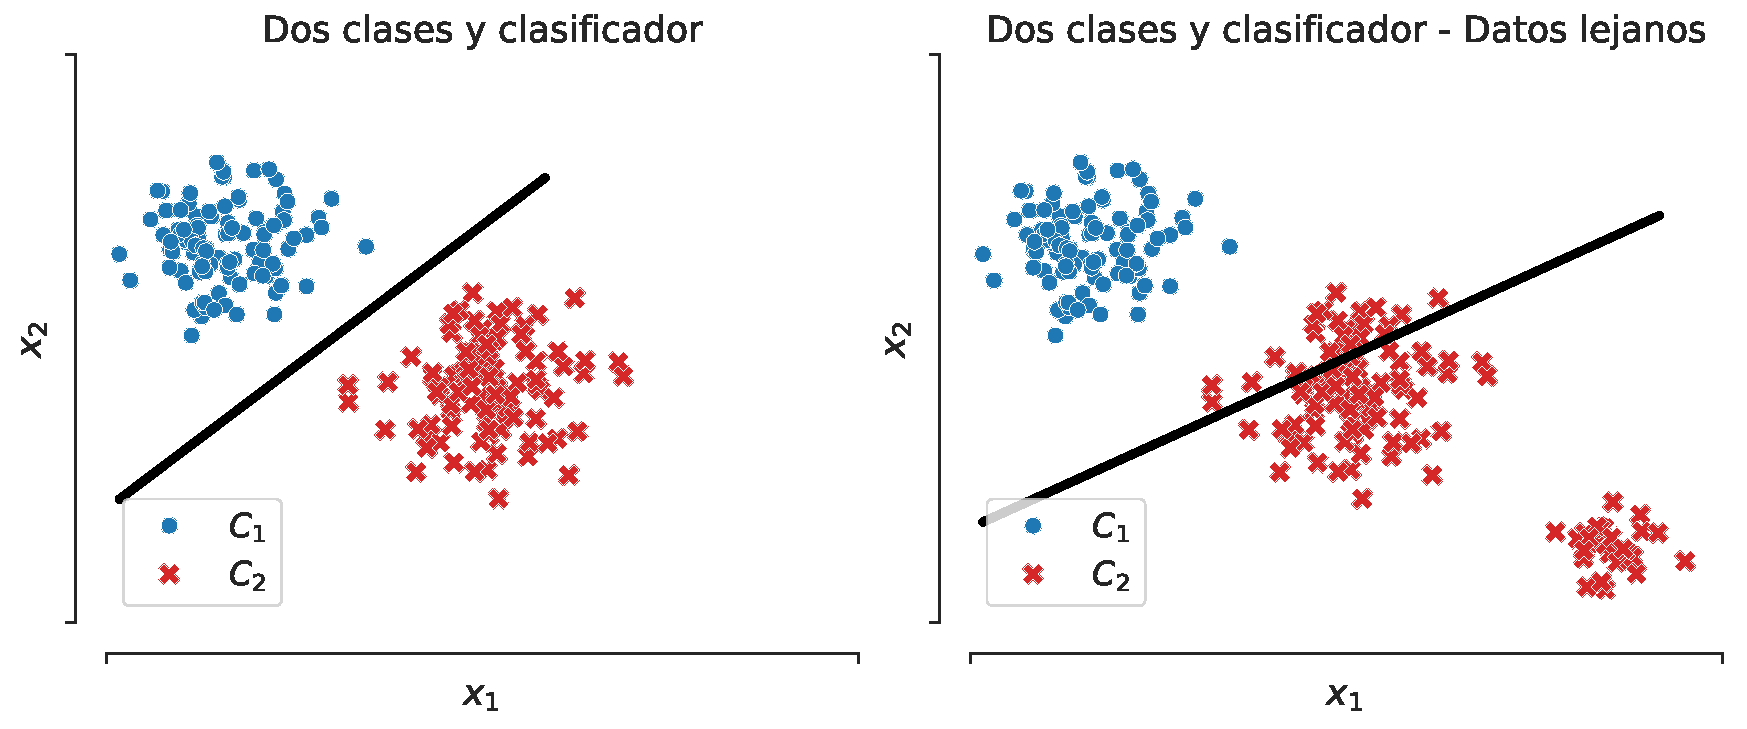
\includegraphics[width=0.8\textwidth]{img/cap3_dosclases_clasificador.pdf}\\
	\caption{Ejemplo ilustrativo sobre cómo los puntos lejanos de una clase pueden afectar incorrectamente los resultados.}
	\label{fig:clasif_mse}
\end{figure}

\subsubsection{El perceptrón}

Las nociones básicas que hemos visto hasta ahora para lidiar con el problema de clasificación tienen dos problemas conceptuales. El primero es la falta de una métrica correcta para evaluar la bondad de nuestro modelo,  esto es porque el criterios de mínimos cuadrados no es apropiado en la evaluación de una asignación de clases, donde no hay concepto de ``más cerca'', sino que solo correcto/incorrecto. Además, todos los enfoques considerados en esta sección hasta este punto no tienen una \emph{función de verosimilitud} apropiada que conecte el modelo (variables latentes) con la clase (observación) de forma coherente. Por el contrario, hasta ahora hemos considerado que por un lado tenemos el modelo lineal para clasificación y por otro lado está \emph{nuestra decisión} de la clase en base a la salida del modelo linear, por  ejemplo si $y(x)>b$ decimos que $x$ pertenece a la clase $\cC_1$.\\

La incorporación de esta función que conecta el modelo lineal con la clase, resulta en un \emph{modelo lineal generalizado}, es decir, una modelo lineal conectado a una  función no-lineal que llamaremos \emph{función de enlace}. Sin embargo, el desafío más importante en esta construcción es que el modelo resultante ya no es lineal, ni en la entrada ni en los parámetros, pues una verosimilitud (función de enlace) lineal nunca nos llevará de un espacio de inputs (hemos asumido $\R^M$) al espacio de categorías $\{\cC_1,\cC_2,\ldots,\cC_k\}$, es decir, necesitamos una no-linealidad ``después'' de la parte lineal, no antes como en el caso de los modelos lineales en lo parámetros vistos en la sección de regresión no lineal.\\

Una forma de resolver estas problemáticas es mediante el uso del \emph{Perceptrón} \cite{rosenblatt_1958}, un modelo de clasificación binario que tuvo mucha importancia en el área de reconocimiento de patrones. El Perceptrón consiste en una función no lineal fija usada para transformar $x$ en un vector de características\footnote{En este caso consideramos no linealidad antes y después de la parte lineal, sin embargo, considerar la entrada como $x$ o  como $\phi(x)$ es  equivalente en base a lo  visto en los modelos lineales en los parámetros. } $\phi(x)\in\R^D$, que luego es usado para generar un modelo lineal \emph{generalizado} con función de enlace no lineal $f(\cdot)$ de la siguiente forma:
\begin{align}
	y(x) &= f(\theta^\top\phi(x))\\
	f(u) &= \left\{\begin{matrix}
	+1,\quad u\geq 0\\
	-1,\quad u<0
	\end{matrix}\right.
\end{align}
Opciones típicas para el vector $\phi(x)$ es concatenar la entrada con un intercepto para la recta, es decir $\phi(x) = [x^\top, 1]$ y $\theta \mapsto [\theta,b]^\top$ como vimos al comienzo del curso, o bien características no lineales como las vistas en la sección de regresión no lineal. El Perceptrón entonces asigna $x$ a la clase $\mathcal{C}_1$ si $y(x)=+1$ y asignará $x$ a la clase $\mathcal{C}_2$ cuando $y(x)=-1$. Notemos que  para  el caso que $\phi$ es lineal, este es el mismo clasificador presentado en la Sección \ref{sec:clasif_lineal}, pero en este caso el criterio para asignar la clase es \textbf{parte del modelo}.\\

Una condición para determinar el parámetro $\theta\in\R^D$ en base a un conjunto de datos  $\datos = \{(x_i,t_i)\}_{i=1}^N$, es que para $x\in\mathcal{C}_1$ ($t=1$), se cumpla que $\theta^\top\phi(x) > 0$, y para $x\in\mathcal{C}_2$ ($t=-1$) se cumpla $\theta^\top \phi(x) < 0$. Usando el hecho que las etiquetas están representadas por la  codificación $t\in\{1,-1\}$, ambas condiciones pueden ser cubiertas por la expresión:
\begin{equation}
	\theta^\top\phi(x_n)t_n > 0,\quad \forall (x_n,t_n) \in \datos.
\end{equation}

Podemos entonces satisfacer esta restricción mediante el ``criterio del perceptrón'', el cual se basa en examinar  los elementos de $\datos$ que fueron clasificados incorrectamente. Este criterio asocia a los puntos clasificados correctamente error 0 y a los puntos mal clasificados error $-\theta^\top\phi(x)t>0$. De esta forma, si denotamos $\mathcal{M}$ el conjunto de puntos mal clasificados, se debe minimizar la siguiente función objetivo:


\begin{equation}
	J_\text{P}(\theta,x) = \E\left(-\theta^\top\phi(x)t(x)\mathds{1}_{\theta^\top\phi(x)t(x)\leq 0} \right) \approx -\sum_{(x_i,t_i)\in \mathcal{D}}\theta^\top\phi(x_i)t_i \mathds{1}_{\theta^\top\phi(x_i)t_i\leq 0} = -\sum_{(x_i,t_i)\in \mathcal{M}}\theta^\top\phi(x_i)t_i
\end{equation}

Para la minimización de dicho funcional, se utilizará un método no determinístico que funciona mejor que el método del gradiente clásico (ver anexos) para este tipo de funciones.


\begin{mdframed}[style=pendiente, frametitle={\center Método del gradiente estocástico}]

	En aprendizaje de máquinas por lo general se busca un parámetro óptimo que minimice el error de ajuste de acuerdo a una función de pérdida $J$. Dicho problema puede ser escrito de la forma:
	
	\begin{equation}
		\hat{\theta} = \argmin_\theta \sum_{i=1}^n J(y_i,\hat{y}_\theta(x_i) = \argmin_\theta \frac{1}{n} \sum_{i=1}^n J(y_i,\hat{y}_\theta(x_i))
	\end{equation}
	
	Donde $y_i$ corresponde a la salida de $x_i$ mientras que $\hat{y}_\theta(x_i))$ representa la predicción de la salida de $x_i$ mediante un modelo de parámetro(s) $\theta$.\\
	
	Muchas veces es infactible encontrar el óptimo de forma analítica o bien, el algoritmo del gradiente clásico se queda atrapado en mínimos locales. Una forma distinta de ver el problema es considerar que $(x_i,y_i)\sim\mu$ iid para una distribución $\mu$ desconocida. Desde ese punto de vista, el problema se reduce a minimizar $\E\left(J(y,\hat{y}_\theta(x))\right)$. Este tipo de problemas puede ser escrito en general como
	
	\begin{equation}
		\min_\theta \E(f(\theta,X)),\quad X\sim \mu\text{ desconocida}
	\end{equation}

Una alternativa al método del gradiente clásico $\theta^{\tau+1} = \theta^\tau - \beta_{\tau+1}\nabla_\theta \E(f(\theta^\tau,X))$ consiste en utilizar las observaciones iid $(x_i)_{i\geq 1}\sim\mu$ al momento de iterar, considerando una observación por iteración en vez del funcional $\E(f(\theta^\tau,X))$ completo, es decir:

\begin{equation}
	\theta^{\tau+1} = \theta^\tau - \eta_{\tau+1}\nabla_\theta f(\theta^\tau,x_{\tau+1})
\end{equation}

Donde ahora $\eta_\tau$ no necesariamente se debe calcular mediante otro problema de minimización, sino que pueden usarse secuencias heurísticas que en la práctica funcionan bien. Además, en cada iteración se necesita evaluar una sola vez $\nabla_\theta f$ y no hace falta calcular su esperanza.\\

Este método es conocido como método del gradiente estocástico (SGD), donde el término $\nabla_\theta f(\theta^\tau,x_{\tau+1})$ puede ser visto como un gradiente exacto perturbado:

\begin{equation}
	\nabla_\theta f(\theta^\tau,x_{\tau+1}) = \nabla_\theta\E(f(\theta^\tau,X)) + \Delta_t
\end{equation}

Donde $\Delta_t = \nabla_\theta f(\theta^\tau,x_{\tau+1}) - \nabla_\theta \E( f(\theta^\tau,X))$ cumple que $\E(\Delta_t)=0$ ya que de acuerdo a la regla integral de Leibniz, $\nabla_\theta \E( f(\theta^\tau,X)) =  \E(\nabla_\theta f(\theta^\tau,X))$.\\


Esta propiedad del gradiente con ruido es la que le permite al algoritmo del gradiente estocástico poder saltarse con mayor facilidad los mínimos locales ya que la evolución de $\theta_\tau$ contiene una parte aleatoria que no depende del valor del gradiente en el punto.


\begin{figure}[H]
	\centering
	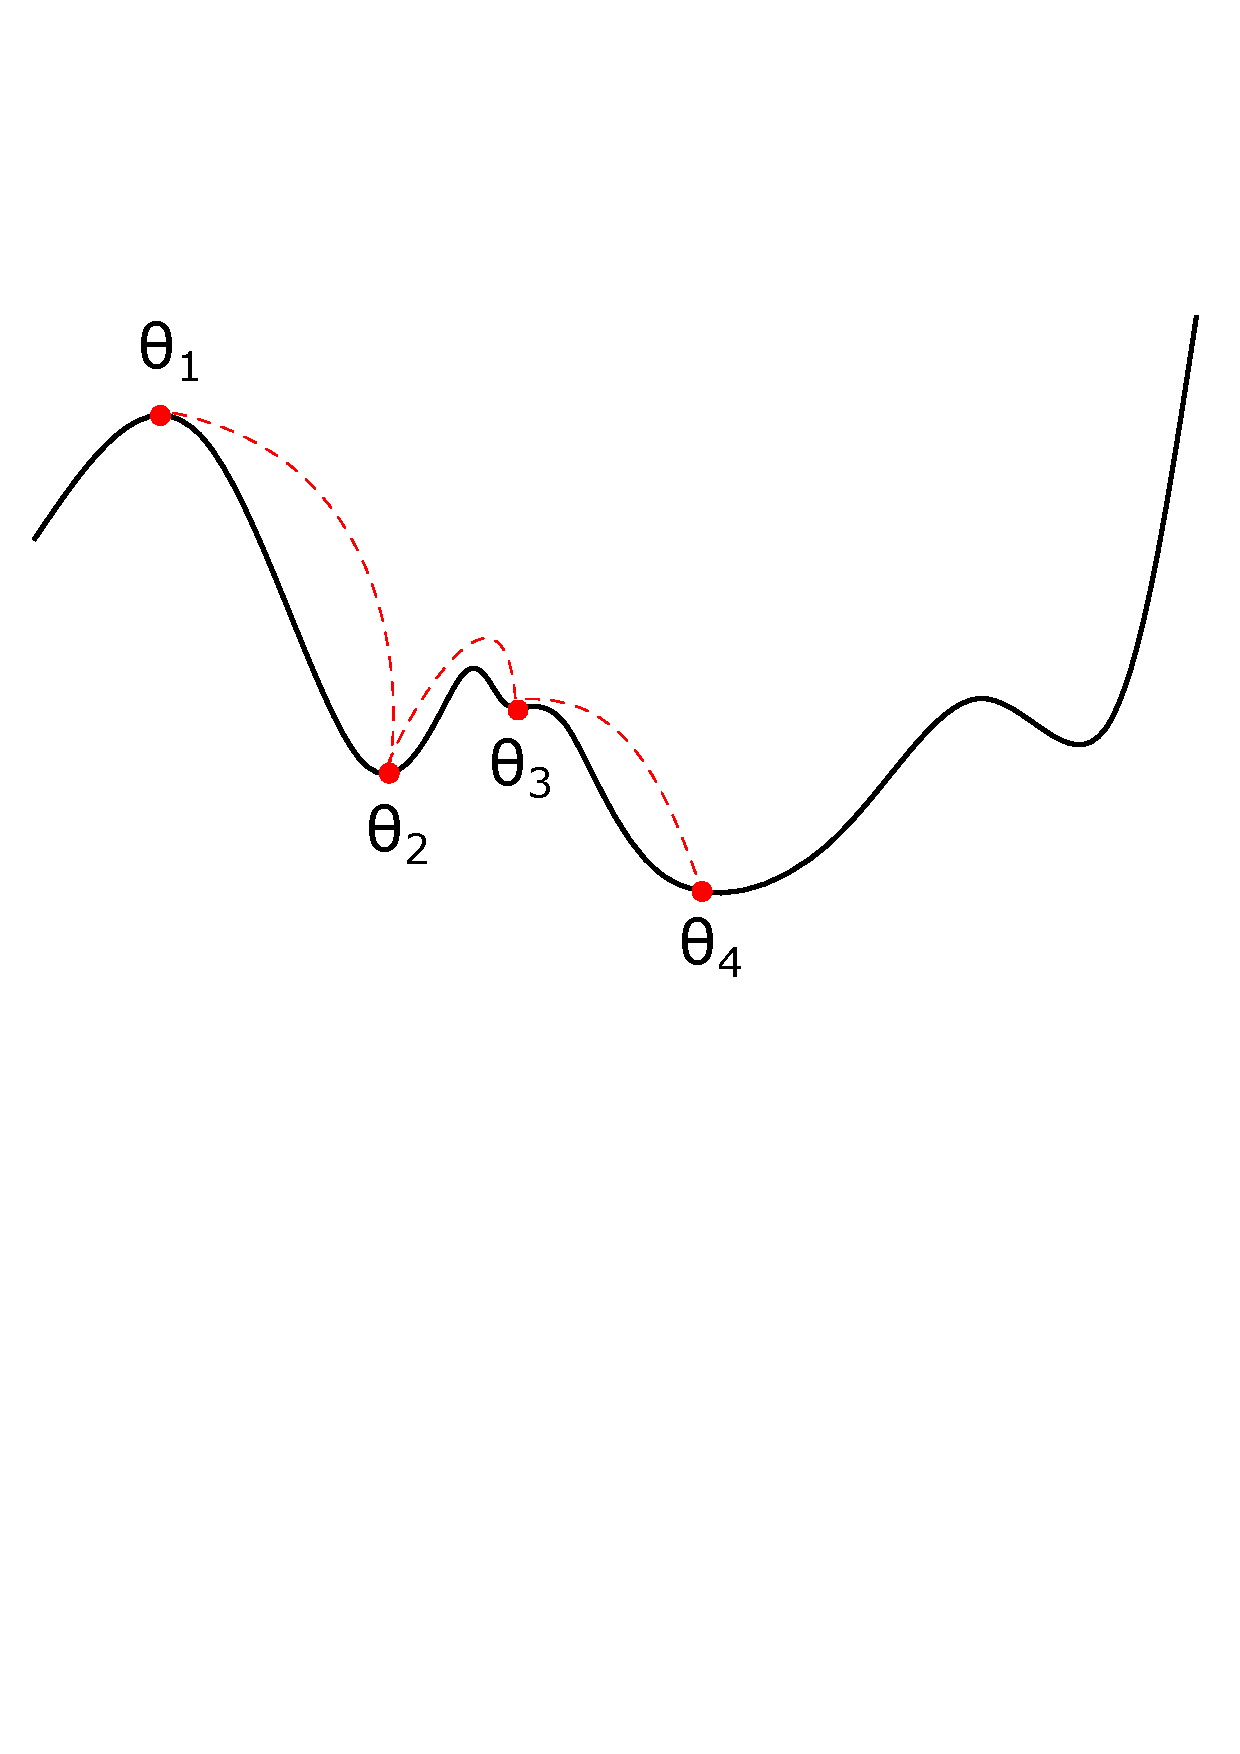
\includegraphics[width=0.6\textwidth]{img/cap3_sgd.pdf}\\
	\caption{Posibles iteraciones del algoritmo SGD. El algoritmo del gradiente clásico hubiese quedado atrapado en $\theta_2$ ya que en dicho punto el gradiente es nulo por lo que no hay desplazamiento.}
\end{figure}

Otra de las ventajas que tiene este algoritmo es que permite entrenar modelos con datos a medida que van llegando (actualización en tiempo real) y no hace falta calcular el funcional de optimización utilizando todos los datos anteriores.\\

Si bien no está garantizada la convergencia a un óptimo global, este método funciona bien en la práctica mediante secuencias probadas de $(\eta_\tau)$ (learning rate). Una selección usual es usar $\eta_\tau$ constante o constante por tramos.\\

Un resultado teórico simple acerca del SGD es el siguiente:


	\begin{theorem}[Sigmund-Robins] Bajo hipótesis razonables sobre $f$ (regularidad en $\theta$, integrabilidad de $\nabla_\theta f$ y cotas) y tasas de aprendizaje suficientemente pequeñas (por ejemplo, $\eta_\tau = 1/\tau$), la sucesión $(\theta^\tau)_{\tau\geq 1}$ converge c.s. al conjunto de puntos críticos de $\E(f(\theta,X))$.\\		
	\end{theorem}
	
En particular, para $f$ convexa, la sucesión converge al conjunto de argumentos minimizantes de $\E(f(\theta,X))$.
	
\end{mdframed}

Para el problema de minimización del funcional del perceptrón, se puede utilizar el método del gradiente estocástico. En este caso, el algoritmo iterativo tiene la siguiente estructura:


\begin{align}
	\theta^{\tau+1} &= \theta^\tau - \eta_\tau \nabla_\theta J_\text{P}(\theta^\tau,x_i)\nonumber\\
	&= \theta^\tau + \eta_\tau \phi(x_i)t_i.\label{eq:percetron_rule}
\end{align}

Es importante notar que al actualizar el vector $\theta$, el conjunto de puntos mal clasificados $\mathcal{M}$ va a cambiar, pues (esperamos que) en cada iteración los elementos del conjunto de puntos mal clasificados vaya disminuyendo.\\

Por lo tanto, el algoritmo de entrenamiento para el perceptrón es el siguiente:

\begin{itemize}
	\item[i)] se recorre el conjunto de puntos de entrenamiento $\{x_i\}_{i=1}^N$,
	\item[ii)] si el punto $x_i$ fue clasificado correctamente el vector de pesos de mantiene igual
	\item[iii)] si $x_i$ fue clasificado incorrectamente, el vector $\theta^\tau$ es actualizado según la ec.~\eqref{eq:percetron_rule} con $\eta=1$ mediante
	\begin{equation}
	 \theta^{\tau+1} = \theta^\tau + \phi(x_i)t_i.
\end{equation}
\end{itemize}
Es decir, el parámetro $\theta$ está paso a paso modificado en la dirección de las características $\phi(x_i)$ con multiplicador $\pm1$ en base a la clase verdadera de $x_i$ hasta  que todos los puntos de $\datos$ están bien clasificados. 




\subsection{Clasificación probabilística: modelo generativo}

Los modelos que hemos revisado hasta este punto son del tipo \emph{discriminativo}, es decir, modelan directamente la función $f:x\mapsto c$. Con una interpretación probabilística, esto es equivalente a modelar la probabilidad condicional $\mathbb{P}(\mathcal{C}_k|x)$, es decir, dado que conozco el input (o características de) $x$, cuál es la distribución de probabilidad sobre las clases. Sin embargo, hemos considerado métodos determinísticos, que solo asignan probabilidad 1 a una sola clase. 


Un paradigma alternativo es considerar es un enfoque \emph{generativo}, en el cual modelamos dos  objetos: en primer lugar la ``probabilidad condicional de clase'' la cual representa cómo distribuyen los valores de los inputs $x$ cuando la  clase es, por  ejemplo, $\cC_k$, denotada por $\mathbb{P}(x|\mathcal{C}_k)$. En segundo lugar las ``probabilidades de clase'', o el prior sobre clases, denotada $\mathbb{P}(\mathcal{C}_k)$. Luego, podemos calcular la densidad posterior sobre las clases dado un input $x$ usando el Teorema de Bayes de acuerdo a 
\begin{equation}
	\mathbb{P}(\mathcal{C}_k|x) = \frac{\mathbb{P}(x|\mathcal{C}_k)\mathbb{P}(\mathcal{C}_k)}{\mathbb{P}(x)}.
\end{equation}

Para el caso de 2 clases, es posible calcular la probabilidad de la clase $\cC_1$ dado $x$ de la forma:
\begin{align}
	\mathbb{P}(\mathcal{C}_1|x) 
	&= \frac{\mathbb{P}(x|\mathcal{C}_1)\mathbb{P}(\mathcal{C}_1)}{\mathbb{P}(x)}\nonumber\\
	&= \frac{\mathbb{P}(x|\mathcal{C}_1)\mathbb{P}(\mathcal{C}_1)}{\mathbb{P}(x|\mathcal{C}_1)\mathbb{P}(\mathcal{C}_1)+\mathbb{P}(x|\mathcal{C}_2)\mathbb{P}(\mathcal{C}_2)}\nonumber\\
	&=\frac{1}{1+\frac{\mathbb{P}(x|\mathcal{C}_2)\mathbb{P}(\mathcal{C}_2)}{\mathbb{P}(x|\mathcal{C}_1)\mathbb{P}(\mathcal{C}_1)}}\nonumber\\
	&=\frac{1}{1+\exp(-r)} = \sigma(r).\label{eq:logistic1}
\end{align}
Donde hemos introducido la notación $r = r(x) =\ln\left(\frac{\mathbb{P}(x|\mathcal{C}_1)\mathbb{P}(\mathcal{C}_1)}{\mathbb{P}(x|\mathcal{C}_2)\mathbb{P}(\mathcal{C}_2)}\right)$  y la  función logística definida mediante $\sigma(r) = \frac{1}{1+e^{-r}}$, la cual  tiene propiedades que serán útiles en el entrenamiento, en particular:
\begin{align}
	\text{reflejo: }\sigma(-r)&=1-\sigma(r)\\
	\text{derivada: }\frac{d}{dr}\sigma(r)&=\sigma(r)(1-\sigma(r))\\
	\text{inversa: }r(\sigma)&=\ln\left(\frac{\sigma}{1-\sigma}\right).
\end{align}


\begin{remark} Si bien la expresión de la distribución condicional en la ec.~\eqref{eq:logistic1} parece una presentación antojadiza para hacer aparecer la  función logística (sigmoide), pues $r=r(x)$ puede ser cualquier cosa. Sin embargo, veremos que existe una elección particular de las distribuciones condicionales de clase que lleva a un $r$ que es efectivamente lineal en $x$. En general, nos  referiremos a este clasificador como \textbf{regresión logística} en dicho caso, es decir, cuando $r(x) = a^\top x  + b$.
\end{remark} 

Podemos ahora considerar el caso de múltiples clases $\{\cC_1,\ldots,\cC_K\}$, donde un desarrollo similar al anterior resulta en:  
\begin{equation}
	\mathbb{P}(\mathcal{C}_i | x) = \frac{\mathbb{P}(x | \mathcal{C}_i)\mathbb{P}(\mathcal{C}_i)}{\sum_{j}\mathbb{P}(x | \mathcal{C}_j)\mathbb{P}(\mathcal{C}_j)} = \frac{\exp(s_i)}{\sum_{j}\exp(s_j)},\label{eq:softmax1}  
\end{equation}
donde hemos denotado $s_i = \log\left(\mathbb{P}(x | \mathcal{C}_i)\mathbb{P}(\mathcal{C}_i)\right)$. La función que aparece al lado derecho de la  ec.~\eqref{eq:softmax1} se conoce como \emph{exponencial normalizada} o \emph{softmax}, y corresponde a una generalización de la función logística a múltiples clases. Además, esta función tiene la propiedad de ser una aproximación suave de la función máximo y convertir cualquier vector $s=[s_1,\ldots,s_k]$ en una distribución de probabilidad, donde podemos hablar de ``la probabilidad de ser clase $\cC_k$''.

\subsubsection{Regresión logística} 
\label{sub:reg_log}

Analizaremos ahora  los supuestos sobre el modelo generativo (i.e., las  probabilidades de clase y condicionales) para encontrar un $r$ --en la ec.~\eqref{eq:logistic1}-- que resulta en la bien conocida regresión logística. Consideraremos el caso binario donde las densidades condicionales de clase son Gaussianas multivariadas, dadas por
\begin{equation}
	p(x|\mathcal{C}_k) \sim \mathcal{N} (\mu_k,\Sigma) = \frac{1}{(2\pi)^\frac{D}{2}|\Sigma|^\frac{1}{2}}\exp(-\frac{1}{2}(x-\mu_k)^\top \Sigma^{-1}(x-\mu_k))\quad k\in\{1,2\}.
\end{equation}

Donde $u_k\in\R^M$ corresponde al centroide de la clase $\mathcal{C}_k$ y $\Sigma\in\R^{M\times M}$ simétrica y definida positiva, corresponde a la matriz de covarianza de las clases (misma matriz para todas las clases). Para este caso, se tiene que para la ecuación \eqref{eq:logistic1}:

\begin{align}
r &= \ln\left(\frac{\mathbb{P}(x|\mathcal{C}_1)\mathbb{P}(\mathcal{C}_1)}{\mathbb{P}(x|\mathcal{C}_2)\mathbb{P}(\mathcal{C}_2)}\right) = \ln\left(\frac{\exp(-\frac{1}{2}(x-\mu_1)^\top \Sigma^{-1}(x-\mu_1))\mathbb{P}(\mathcal{C}_1)}{\exp(-\frac{1}{2}(x-\mu_2)^\top \Sigma^{-1}(x-\mu_2))\mathbb{P}(\mathcal{C}_2)}\right)\\
&= -\frac{1}{2}(x-\mu_1)^\top \Sigma^{-1}(x-\mu_1) +\frac{1}{2}(x-\mu_2)^\top \Sigma^{-1}(x-\mu_2) + \ln\left(\frac{p(\mathcal{C}_1)}{p(\mathcal{C}_2)}\right)\\
&= \frac{1}{2}\left(x^\top\Sigma^{-1}(\mu_1-\mu_2) + (\mu_1-\mu_2)^\top\Sigma^{-1}x - \mu_1\Sigma^{-1}\mu_1 + \mu_2\Sigma^{-1}\mu_2 \right) + \ln\left(\frac{p(\mathcal{C}_1)}{p(\mathcal{C}_2)}\right)\\
&= (\mu_1-\mu_2)^\top\Sigma^{-1}x + \frac{1}{2}\left(\mu_2\Sigma^{-1}\mu_2 - \mu_1\Sigma^{-1}\mu_1 \right)+ \ln\left(\frac{p(\mathcal{C}_1)}{p(\mathcal{C}_2)}\right)\\
&= a^\top x+b
\end{align}

donde hemos usado la notación
\begin{align}
a &= \Sigma^{-1}(\mu_1-\mu_2)\\
b &= \frac{1}{2}(\mu_2^\top \Sigma^{-1}\mu_2-\mu_1^\top \Sigma^{-1}\mu_1)
+\ln\left(\frac{p(\mathcal{C}_1)}{p(\mathcal{C}_2)}\right). 
\end{align}

y el hecho de que $\Sigma^{-1}$ es simétrica.\\

Lo anterior nos entrega la regresión logística (lineal) para el  caso binario, donde al incorporar la expresión anterior en la ec.~\eqref{eq:logistic1} obtenemos
\begin{equation}
	p(\mathcal{C}_k|x) = \sigma(a^\top x+b) = \frac{1}{1 + \exp{\left(-a^\top x-b\right)}}. \label{eq:logistica2}
\end{equation}

\begin{remark}
	La reducción de $r$ a una forma lineal prueba que es necesario considerar matrices de covarianza $\Sigma$ iguales para todas las clases, ya que de lo contrario no se podrían simplificar los términos cuadráticos $x^\top\Sigma^{-1}x$.
\end{remark}

\begin{remark}\label{rem:reg_log} 
El modelo de clasificación binaria en la  ec.~\ref{eq:logistica2} es conocido como \emph{regresión logística} y es la consecuencia de asumir un modelo generativo Gaussiano con distintas medias pero la misma varianza para una de las clases. Como consecuencia, la región de decisión se encuentra imponiendo que la probabilidad de ser clase $\cC_1$ sea 1/2 (y por ende, ser $\cC_2$ también tiene probabilidad 1/2), lo cual se tiene para 
\begin{equation}
	a^\top x+b = 0.
\end{equation}
\end{remark}

Ahora que hemos definido el modelo para nuestro problema de clasificación, aflora naturalmente la siguiente pregunta: ¿Cómo ajustar los parámetros de las condicionales a la clase y priors respectivamente? Para esto, reiteremos que los parámetros del modelos serán los de la probabilidad de clase $p(\cC_k)$ y de la probabilidades condicionales de clase $p(x|\cC_k)$. Respectivamente: 

\begin{itemize}
	\item Probabilidad de clase:
	\begin{equation}
	 	p(\mathcal{C}_1)=\pi,\quad  p(\mathcal{C}_2)=1-\pi,\label{eq:prob_clase}
	 \end{equation}  es decir,  un parámetro $\pi$ (por determinar).
	\item Probabilidad condicional de clase:
	\begin{equation}
		p(x|\mathcal{C}_k) = \mathcal{N}(\mu_k,  \Sigma); k=1,2,\label{eq:prob_clase_cond}
	\end{equation} 
	es decir, parámetros $ \mu_1\in\R^M,\mu_2\in\R^M,\Sigma\in\R^M\times\R^M$ (por determinar) o, equivalentemente, $M + M + M(M+1)/2=M(M+5)/2$ parámetros escalares (considerando que $\Sigma$ es simétrica). 
\end{itemize}
Denotaremos todos los parámetros mediante el parámetro agregado $\theta =\{\pi,\mu_1,\mu_2,\Sigma \}$.\\

Realizaremos el entrenamiento del modelo, i.e., encontrar $\theta$ en base a un conjunto de datos $\datos$, mediante el método de máxima verosimilitud. Para esto, notemos que solo hemos definido ``la probabilidad de ser clase $\cC_1$'', noción que extendemos usando la codificación de clases $t\in\{0,1\}$.  Con esta codificación, donde la observación $(x_i,t_i)$ corresponde a clase $\cC_1$ con $t_i = 1$ y a clase $\cC_2$ con  $t=0$, podemos expresar la verosimilitud con una observación mediante:
\begin{equation}
	L_i(\theta) = p(x_i, t_i|\theta) =  p(x_i,\cC_1|\theta)^{t_i}p(x_i,\cC_0|\theta)^{1-t_i}. 
\end{equation}
Esta expresión equivale a la probabilidad de ser clase $\cC_1$ cuando $t_i=1$ y a la probabilidad de ser clase $\cC_0$ cuando $t_i=0$. Consecuentemente, para un conjunto de datos $\datos$ de la forma

\begin{equation}
X=\left(\begin{matrix}
		x_1^\top\\ \vdots\\ x_N^\top
	\end{matrix}\right)\in\R^{N\times M},\qquad
	T=\left(\begin{matrix}
		t_1\\ \vdots\\ t_N
	\end{matrix}\right)\in\{0,1\}^N \text{ es decir, codificación $0-1$.}
\end{equation}

podemos escribir la verosimilitud mediante $L(\theta) = p(X,T|\theta) $, luego:
\begin{align}
	L(\theta) &= \prod_{i=1}^{N}p(x_i,t_i|\theta)
	= \prod_{i=1}^{N}p(x_i,\mathcal{C}_1|\theta)^{t_i}p(x_i,\mathcal{C}_0|\theta)^{1-t_i}\\
	&=\prod_{i=1}^{N}\left(p(x_i|\mathcal{C}_1,\theta)p(\mathcal{C}_1|\theta)\right)^{t_i}\left(p(x_i|\mathcal{C}_0,\theta)p(\mathcal{C}_0|\theta)\right)^{1-t_i}\\
	&= \prod_{i=1}^{N}(\pi\mathcal{N}(x_i|\mu_1,\Sigma))^{t_i}
	((1-\pi)\mathcal{N}(x_i|\mu_2,\Sigma))^{1-t_i}.
	\end{align}

Al igual que en el escenario de regresión lineal, para proceder con la optimización nos enfocamos en la log-verosimilitud, dada por:	
	\begin{equation}
	l(\theta) := \log L(\theta) = \sum_{i=1}^{N}\left(t_i(\log(\pi)+\log(\mathcal{N}(x_i|\mu_1,\Sigma)))+(1-t_i)(\log(1-\pi)+\log(\mathcal{N}(x_i|\mu_2,\Sigma)))\right) 
		\end{equation}

Aplicando entonces las condiciones de primer orden, tenemos que 
\begin{itemize}
	
\item \textbf{1)} Con respecto a $\pi$:
	
	\begin{align}
	\frac{\partial\log(L)}{\partial\pi} &= \sum_{i=1}^N \frac{t_i}{\pi}-\frac{1-t_i}{1-\pi}=0\nonumber\\
	\Rightarrow \quad & (1-\pi)\sum_{i=1}^Nt_i = \pi\sum_{i=1}^N(1-t_i)\nonumber\\
	\Rightarrow \quad & \sum_{i=1}^Nt_i=\pi N \quad\Rightarrow\quad \pi = \frac{\sum_{i=1}^Nt_i}{N} = \frac{N_1}{N_1+N_2} \label{eq:log_reg_pi}
	\end{align}
	
	Donde $N_i:=\text{Card}(x:x\in\mathcal{C}_i)$. Por lo tanto, el EMV de $pi$ colapsa a la regla de Laplace.
	
\item \textbf{2)} Con respecto a $\mu_1$:
	
	\begin{align}
	\frac{\partial\log(L)}{\partial\mu_1} &= \sum_{i=1}^N t_i
	\frac{\partial}{\partial \mu_1}(-\frac{1}{2}(x_i-\mu_1)^\top \Sigma^{-1}(x_i-\mu_1))\nonumber\\
	&= \sum_{i=1}^N t_i(\Sigma^{-1}(x_i-\mu_1)) =
	\Sigma^{-1}\sum_{i=1}^N t_i(x_i-\mu_1) = 0\nonumber\\
	\Rightarrow\quad & \sum_{i=1}^Nt_ix_i= \mu_1\sum_{i=1}^N t_i
	\quad\Rightarrow\quad \mu_1  = \frac{1}{N_1}\sum_{i=1}^Nt_ix_i = \frac{1}{N_1}\sum_{x_i\in \mathcal{C}_1}x_i \label{eq:log_reg_mu1}
	\end{align}
	
	De forma análoga:
	\begin{equation}
	\mu_2 = \frac{1}{N_2}\sum_{x_i\in \mathcal{C}_2}x_i \label{eq:log_reg_mu2}
	\end{equation}
	
\end{itemize}

\begin{remark}\label{rem:log_reg_interpretacion_ML}
La ec.~\eqref{eq:log_reg_pi} revela que el parámetro  óptimo $\pi$ es precisamente la razón entre la cantidad de elementos de la clase $\cC_1$ y el total de datos, esto es porque $\pi$ es la probabilidad de ser clase $\cC_1$; lo mismo aplica para $(1-\pi)$ y clase $\cC_0$. Además, de las ecs.~\eqref{eq:log_reg_mu1}-\eqref{eq:log_reg_mu2} vemos también que el estimador de MV para la media de las clases es la media muestral de los datos disponibles por cada clase. Queda la siguiente pregunta entonces: ¿cuál es el estimador de MV de $\Sigma$?
\end{remark}

\subsubsection{Regresión logística v/s modelo generativo}

Recordemos que los supuestos tomados sobre el modelo generativo para el problema de clasificación resultaron en:
\begin{equation}
p(\mathcal{C}_1|x) = \sigma(w^\top x) = \frac{1}{1+e^{-w^\top x}} \label{eq:log_reg_discriminativo},
\end{equation}
donde por claridad de notación hemos elegido la representación lineal $(w^\top x)$ y no afín $(a^\top x + b)$. 

En el caso anterior se ha entrenado el modelo generativo completo, es decir, $\pi, \mu_1,\mu_2, \Sigma$, lo cual tiene la ventaja de tener solución en forma cerrada, sin embargo, puede ser innecesario cuando solo necesitamos conocer el peso $w$ en la ecuación anterior. Otra forma de entrenar la  regresión logística es considerar el modelo discriminativo en la  ec.~\eqref{eq:log_reg_discriminativo} y optimizar directamente la verosimilitud sobre  este modelo para encontrar $w$; en vez de todos los parámetros $\pi,\mu_1,\mu_2,\Sigma$ del modelo generativo.

Calculemos la verosimilitud de la regresión logística con datos $\datos=\{(x_i,t_i)\}_{i=1}^N$, para hacer la notación más compacta denotamos $\sigma_i = \sigma(w^\top x_i)$. Entonces:
\begin{equation}
p((t_i)_{i=1}^N|(x_i)_{i=1}^N,w) = \prod_{i=1}^{N}p(t_i|x_i,w)= \prod_{i=1}^{N} p(\mathcal{C}_1|x_i)^{t_i} p(\mathcal{C}_2|x_i)^{1-t_i} =  \prod_{i=1}^{N}\sigma_i^{t_i}(1-\sigma_i)^{1-t_i} 
\end{equation}
Con lo que la log-verosimilitud está dada por
\begin{equation}
	l(w) = \sum_{i=1}^N t_i\log(\sigma_i) + (1-t_i)\log(1-\sigma_i).
\end{equation}

Notemos que este  problema de optimización no exhibe una solución en forma cerrada, por lo que podemos resolverlo mediante gradiente, para lo cual es necesario calcular el gradiente de $l(w)$ respecto a $w$:
\begin{align}
\nabla_w l(w) = \sum_{i=1}^N (t_i-\sigma_i)x_i,
\end{align}
lo cual nos da una regla de  ajuste $\theta \mapsto \theta - \eta \sum_{i=1}^N (\sigma_i-t_i)x_i$, o bien 
\begin{equation}
	\theta \mapsto \theta + \eta(t_i-\sigma_i)x_i, \label{eq:reg_log_theta_update}
\end{equation}
si tomamos los  datos de ``a uno'' (método del gradiente estocástico).
\begin{remark}\label{rem:log_reg_shocks}
Notemos que la regla de ajuste del parámetro $\theta$ en la ec.~\eqref{eq:reg_log_theta_update} recuerda el ajuste del Perceptrón en la ec.~\eqref{eq:percetron_rule}, donde los puntos mal clasificados se agregan como características al vector $\theta$. Sin  embargo, a diferencia del  perceptrón, incluso los elementos bien clasificados ($\sigma$  cercano a  1 ó 0) tomarán parte en la actualización, forzando una fuerte componente de sobreajuste al hacer tender $\theta$ a infinito. 
\end{remark}

\begin{figure}[H]
	\centering
	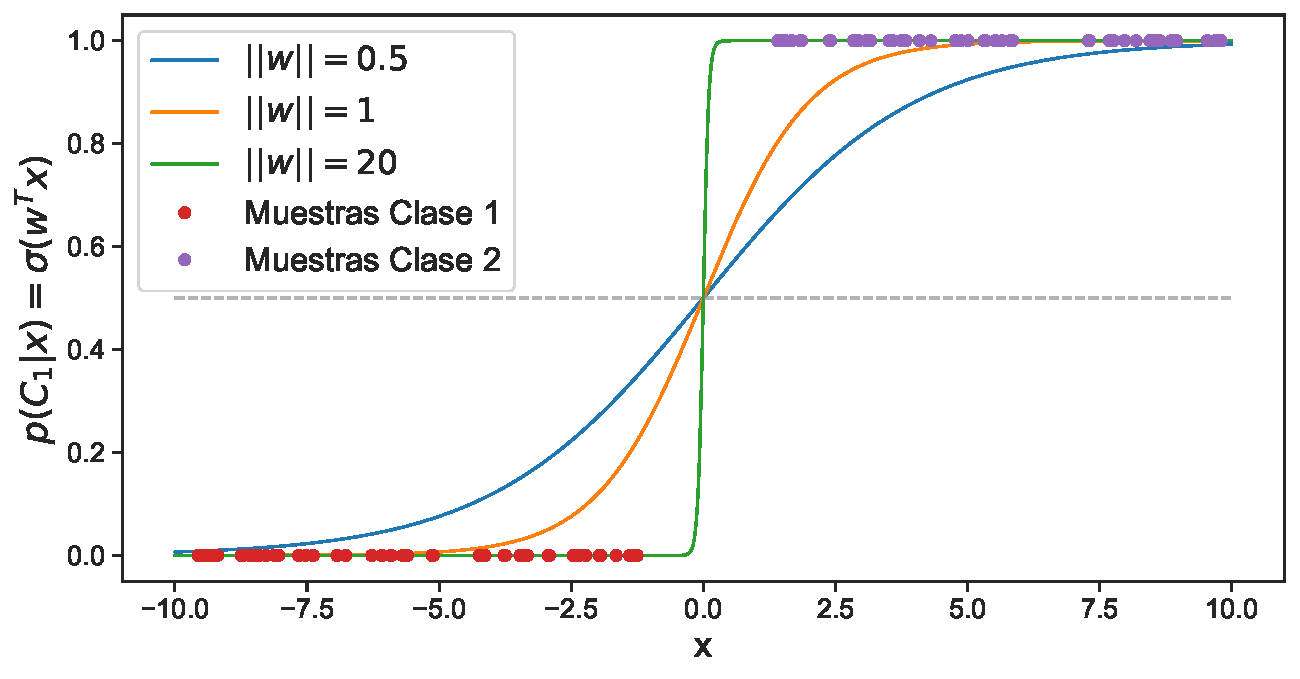
\includegraphics[width=0.9\textwidth]{img/cap3_logistica.pdf}\\
	\caption{En gris la frontera de decisión: una nueva entrada $x_\star$ será asignada a la clase $\cC_1$ si $p(\cC_1|x_\star)>\frac{1}{2}$, en caso contrario, será asignada a $\cC_2$. Se observa que al entrenar con más muestras, $\norm{w}$ crece por lo que el parámetro se sobreajusta a los datos y el clasificador converge a una función indicatriz.}
\end{figure}



